\chapter{عامل بولتزمان}\label{ch:b2:boltzmann-factor}

اصعد جبلًا فيرقّ الهواء: فعلى ثلاثة آلاف متر يهبط
الضغط إلى \qty{0.7}{bar}، وعلى قمة إفرست إلى ثلث
قيمته عند مستوى البحر. ولا شيء يحصر الجوّ من فوق؛ بل
تمسكه الثقالة وينشره الاضطراب الحراري، و
المساومة بينهما أسّية، $n \propto
\eu^{-mgz/k_BT}$ --- فنسبة الطاقة الكامنة للجزيء إلى
$k_BT$ تقرر كم يندر هناك في العلاء. والأسّية نفسها تحكم
نسبة الذرات في مستوٍ مثار، وعدد الجزيئات السريعة
كفاية للإفلات من كوكب، ومغنطة جسم بارامغناطيسي،
والجمهرات التي على الليزر أن يقلبها، والكمّات التي يعدّها قانون بلانك:
وهي \emph{عامل بولتزمان}، وهي أنفع صيغة مفردة
في الفيزياء الإحصائية. وهذا الفصل يسوّغها بالجوّ،
ويذكرها في العام، ويستخرج منها، بمجاميع وتكاملات
غاوسية لا غير، النظامَ ذا المستويين وسعته
الحرارية، وتوزّع الطاقة بالتساوي، وتوزيع سرعات الجزيئات،
\omterm{prop:b2:boltzmann-factor:curie}{وقانون كوري} في البارامغناطيسية --- ومعها، في الطريق، متوسط طاقة
مذبذب كمومي، وهو صيغة بلانك.

\begin{omfigure}
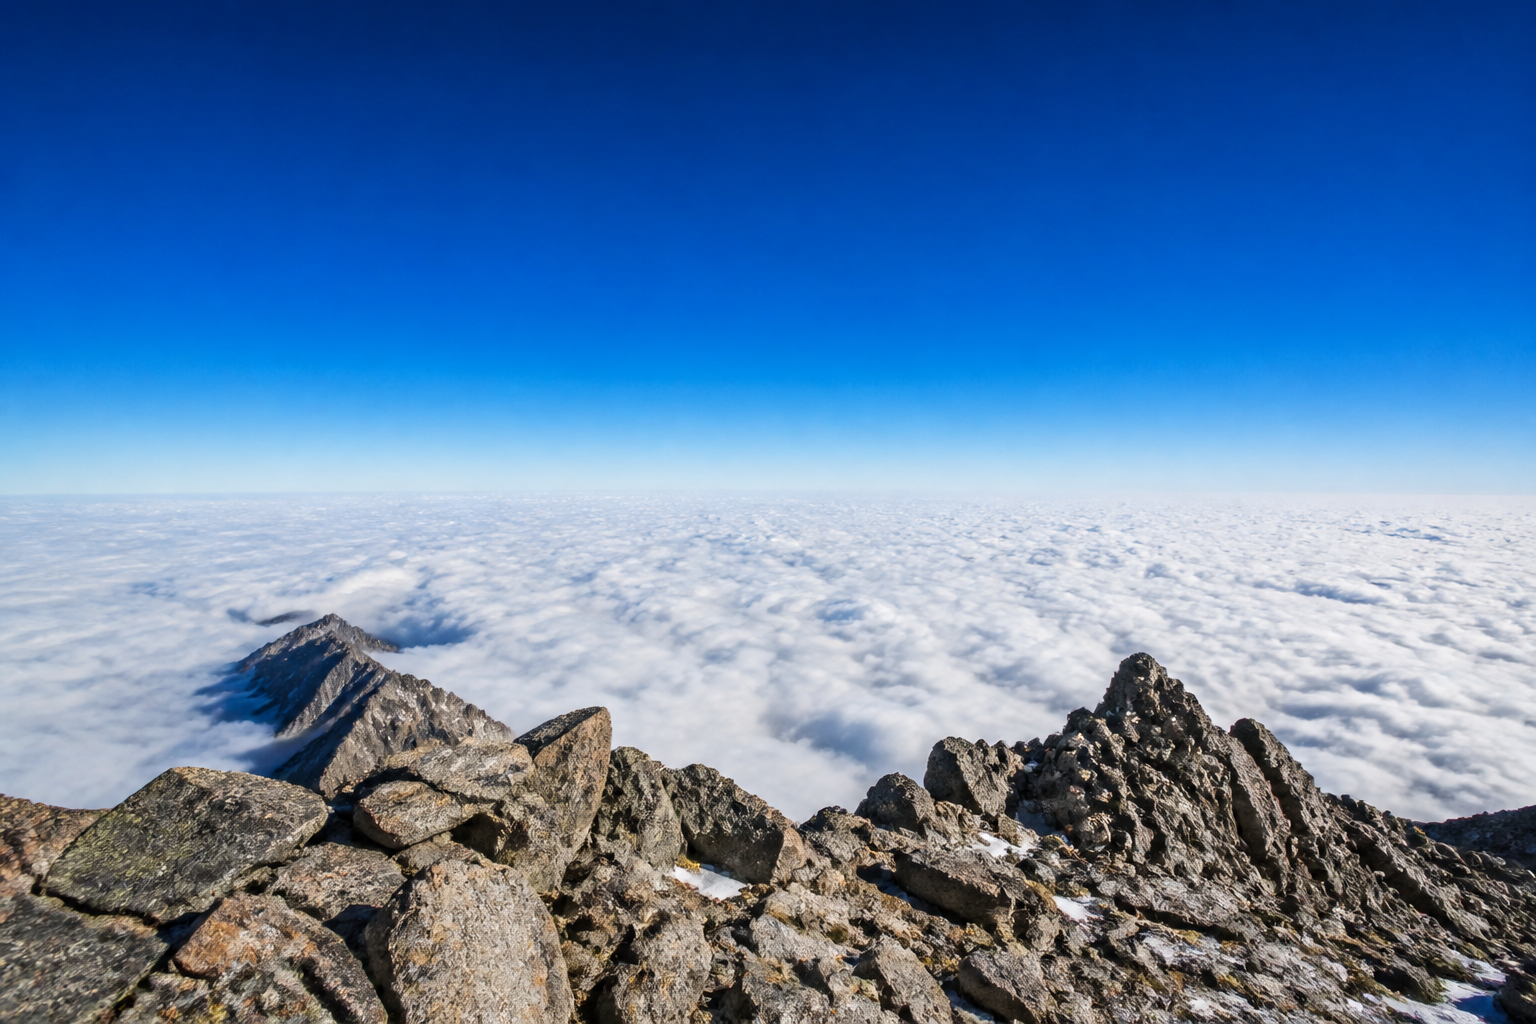
\includegraphics[width=0.58\linewidth]{images/book4/ai/b4-29-sky-gradient-summit.png}

{\small من قمة، ضباب الجوّ الأسفل والزرقة
العميقة فوقه: فكثافة الهواء تهبط بالعامل $\eu$ كل
\qty{8}{km} --- وهو عامل بولتزمان للطاقة الكامنة للجزيء في
ثقالة الأرض.}
\end{omfigure}

\section{الجوّ متساوي الحرارة}

\begin{proposition}[القانون البارومتري]\label{prop:b2:boltzmann-factor:barometric}
في جوّ من غاز مثالي (كتلته الجزيئية $m$) عند حرارة
منتظمة $T$ في ثقالة منتظمة $g$، يهبط الضغط \omterm{def:b2:particle-diffusion:flux}{والكثافة
العددية} أسّيًّا مع الارتفاع:
\[
P(z) = P_0\,\eu^{-z/H}, \qquad n(z) = n_0\,\eu^{-mgz/k_BT}, \qquad
H = \frac{k_BT}{mg} ,
\]
مع \emph{ارتفاع السلّم}\index{ارتفاع السلّم} $H \approx \qty{8.4}{km}$
من أجل الهواء عند \qty{288}{K}. والأسّ هو نسبة الطاقة الكامنة
$mgz$ للجزيء إلى الطاقة الحرارية $k_BT$.
\end{proposition}

\begin{proof}
الهيدروستاتيك، $\dd P/\dd z = -\rho g = -nmg$، وقانون الغاز المثالي $P
= nk_BT$: $\dd P/\dd z = -(mg/k_BT)P$، أي أسّية. والجوّ
الحقيقي يبرد مع الارتفاع (نحو \qty{6.5}{K/km} في أدنى عشرة
كيلومترات)، وذلك يجعل الهبوط أسرع قليلًا؛ والنموذج
متساوي الحرارة جيد في حدود $20\%$.
\end{proof}

\begin{omfigure}
\begin{tikzpicture}
  \begin{axis}[omaxis, width=8.2cm, height=4.8cm, xmin=0, xmax=32, ymin=0, ymax=1.1,
    xlabel={$z$ (\unit{km})}, ylabel={$P/P_0$}, xtick={8.4,16.8,25.2}, xticklabels={$H$,$2H$,$3H$}, ytick={0.37,1}, yticklabels={$1/\eu$,$1$}, clip=false,
    legend style={font=\scriptsize, at={(0.97,0.45)}, anchor=north east, draw=none, fill=none}]
    \addplot[omDef, thick, domain=0:32, samples=80] {exp(-x/8.4)};
    \addlegendentry{الهواء، \qty{288}{K}}
    \addplot[omExo, thick, dashed, domain=0:32, samples=80] {exp(-x/60)};
    \addlegendentry{الهليوم وحده، $H = \qty{60}{km}$}
    \draw[dashed, gray] (axis cs:8.4,0) -- (axis cs:8.4,0.37) -- (axis cs:0,0.37);
  \end{axis}
\end{tikzpicture}

{\small الجوّ متساوي الحرارة: يهبط الضغط والكثافة بالعامل $1/\eu$
في كل \omterm{prop:b2:boltzmann-factor:barometric}{ارتفاع سلّم} $H = k_BT/mg$؛ ولغاز أخفّ $H$ أكبر
--- لكن دون \qty{100}{km} يبقي الاضطراب الهواء ممزوجًا، وتشترك
الغازات كلها في $H$ الوسطي.}
\end{omfigure}

\section{عامل بولتزمان}

\begin{theorem}[عامل بولتزمان]\label{thm:b2:boltzmann-factor:factor}
النظام المتوازن حراريًّا مع منظِّم حراري عند الحرارة
$T$ يوجد في حالة مجهرية معينة طاقتها $E$ باحتمال
متناسب مع
\[
\eu^{-E/k_BT} .
\]
ومن ثَمّ، من أجل مجموعة حالات منفصلة طاقاتها $E_i$،
\[
p_i = \frac{\eu^{-E_i/k_BT}}{Z}, \qquad Z = \sum_i\eu^{-E_i/k_BT} ,
\]
حيث يُنظِّم المجموع $Z$ (وهو \emph{تابع التقسيم}\index{تابع التقسيم})
الاحتمالات؛ وتُعمَر حالتان (أو مستويان متساويا الانحلال)
بالنسبة $N_2/N_1 = \eu^{-(E_2 - E_1)/k_BT}$؛
ومن أجل متغير مستمرّ (موضع، أو سرعة) تكون كثافة
الاحتمال متناسبة مع $\eu^{-E/k_BT}$ في ذلك المتغير. وعند
\qty{300}{K}، $k_BT = \qty{4.1e-21}{J} = \qty{0.026}{eV}$: فكل ما
يكلّف أكثر من هذا بكثير نادر، وكل ما يكلّف أقلّ منه بكثير
يُثار بحرية.
\end{theorem}

\begin{proof}
القانون البارومتري هو العامل من أجل الطاقة الكامنة $mgz$؛ ونقبل
عموميته، لكن هذه هي الحجة (وتُحكَم في مجلد
السنة الثالثة). فالمنظِّم $R$ كبير؛ ومتى كان نظامنا الصغير في
حالة طاقتها $E$، كانت للمنظِّم الطاقة $E_{\text{كلي}} -
E$، وأمكن أن يكون في $\Omega_R(E_{\text{كلي}} - E)$ حالة مجهرية، وكلها
متساوية الاحتمال (وهي المصادرة الأساسية من أجل كلٍّ معزول). ومن ثَمّ
$p(E) \propto \Omega_R(E_{\text{كلي}} - E)$. ومع تعريف بولتزمان
للإنتروبيا، $S_R = k_B\ln\Omega_R$، و $1/T = \dd S_R/\dd E_R$ من أجل
المنظِّم، يكون $\ln\Omega_R(E_{\text{كلي}} - E) \approx \ln\Omega_R(E_{\text{كلي}})
- E/k_BT$ لأن $E \ll E_{\text{كلي}}$؛ ثم خذ الأسّية.
\end{proof}

\begin{example}[جمهرات المستويات الذرية]\label{ex:b2:boltzmann-factor:levels}
يقع أول مستوٍ مثار للهدروجين على \qty{10.2}{eV} فوق الحالة
الأساسية: فعند \qty{300}{K}، $\eu^{-395}$ --- أي ولا ذرة واحدة في الكون؛ وعند
\qty{6000}{K}، وهي حرارة سطح الشمس، $\eu^{-19.7} \approx 3 \times 10^{-9}$ (مضروبًا
في انحلال قدره $4$): وهو كافٍ، في عمود الغاز الشمسي الهائل، من أجل
خطوط امتصاص بالمر، وهي أشدّ ما تكون في النجوم قرب \qty{10000}{K}.
وخط الصوديوم D (\qty{2.1}{eV}) في لهب \qty{2500}{K}: $\eu^{-9.8} = 6
\times 10^{-5}$ من الذرات مثارة، وهو ما يعطي اللهب الأصفر لرشة
ملح. وأما وسط الليزر في \cref{ch:b2:laser}: فالعامل
يقول إن مستواه الأعلى فارغ عند التوازن، وعلى المضخة أن تصارعه.
\end{example}

\section{المستويات المنفصلة: النظام ذو المستويين والمذبذب}

\begin{proposition}[متوسط الطاقة من تابع التقسيم]\label{prop:b2:boltzmann-factor:meanE}
مع $\beta = 1/k_BT$،
\[
\langle E\rangle = \sum_ip_iE_i = -\frac{\partial\ln Z}{\partial\beta}, \qquad
C = \frac{\dd\langle E\rangle}{\dd T} .
\]
\end{proposition}

\begin{proof}
$\partial_\beta Z = -\sum E_i\eu^{-\beta E_i}$، ثم اقسم على $Z$.
\end{proof}

\begin{proposition}[النظام ذو المستويين]\label{prop:b2:boltzmann-factor:twolevel}
$N$ نظامًا مستقلًّا لكلٍّ منها مستويان $0$ و $\varepsilon$ (كسبينات في
حقل، أو ذرات لها مستوٍ مثار واحد، أو عيوب لها موضعان):
\[
\frac{N_2}{N} = \frac{1}{\eu^{\varepsilon/k_BT} + 1}, \qquad
\langle E\rangle = \frac{N\varepsilon}{\eu^{\varepsilon/k_BT} + 1}, \qquad
C = Nk_B\,\frac{x^2\eu^x}{(\eu^x + 1)^2}, \quad x = \frac{\varepsilon}{k_BT} .
\]
والمستوي الأعلى فارغ عند الحرارة المنخفضة وممتلئ إلى النصف على الأكثر عند
الحرارة العالية (فلا ينقلب قط عند التوازن)؛ والسعة الحرارية
تنعدم عند الطرفين وتبلغ قمتها $0.44\,Nk_B$ قرب $k_BT = 0.42
\varepsilon$ --- وهي \emph{شذوذ شوتكي}\index{شذوذ شوتكي}، وهي
بصمة فجوة في الطيف.
\end{proposition}

\begin{proof}
$Z = 1 + \eu^{-x}$؛ و $p_2 = \eu^{-x}/(1 + \eu^{-x})$؛ ثم اشتقّ $\langle
E\rangle$ بالنسبة إلى $T$.
\end{proof}

\begin{omfigure}
\begin{tikzpicture}
  \begin{axis}[omaxis, width=6.4cm, height=4.4cm, xmin=0, xmax=3.2, ymin=0, ymax=1.1,
    xlabel={$k_BT/\varepsilon$}, ylabel={الجمهرتان}, xtick={1,2,3}, ytick={0.5,1}, clip=false]
    \addplot[omDef, thick, domain=0.02:3.2, samples=100] {1/(exp(1/x)+1)};
    \addplot[omExo, thick, domain=0.02:3.2, samples=100] {exp(1/x)/(exp(1/x)+1)};
    \node[font=\scriptsize, omExo] at (axis cs:1.4,0.85) {$N_1/N$};
    \node[font=\scriptsize, omDef] at (axis cs:1.4,0.2) {$N_2/N$};
  \end{axis}
  \begin{axis}[omaxis, width=6.4cm, height=4.4cm, xmin=0, xmax=3.2, ymin=0, ymax=0.55, xshift=6.6cm,
    xlabel={$k_BT/\varepsilon$}, ylabel={$C/Nk_B$}, xtick={1,2,3}, ytick={0.44}, clip=false]
    \addplot[omThm, thick, domain=0.08:3.2, samples=120] {(1/x)^2*exp(1/x)/(exp(1/x)+1)^2};
    \draw[dashed, gray] (axis cs:0.42,0) -- (axis cs:0.42,0.44);
    \node[font=\scriptsize, below] at (axis cs:0.42,0) {$0.42$};
  \end{axis}
\end{tikzpicture}

{\small النظام ذو المستويين: الجمهرتان بدلالة الحرارة (فالمستوي
الأعلى يمتلئ نحو النصف، ولا يتجاوزه) والسعة الحرارية
لشوتكي، وهي نتوء حيث تطابق $k_BT$ الفجوةَ.}
\end{omfigure}

\begin{proposition}[المذبذب الكمومي وصيغة بلانك]\label{prop:b2:boltzmann-factor:oscillator}
لمذبذب توافقي تواتره $\nu$ المستويات $E_n = nh\nu$ (زائدًا
ثابتًا)؛ وعند الحرارة $T$،
\[
Z = \frac{1}{1 - \eu^{-h\nu/k_BT}}, \qquad
\langle E\rangle = \frac{h\nu}{\eu^{h\nu/k_BT} - 1}
\ \longrightarrow\
\begin{cases} k_BT & (h\nu \ll k_BT), \\ h\nu\,\eu^{-h\nu/k_BT} & (h\nu \gg k_BT). \end{cases}
\]
وهذا متوسط طاقة نمط من حقل الإشعاع الذي يضربه قانون
بلانك (\cref{ch:b2:thermal-radiation}) في عدد الأنماط،
وهو متوسط طاقة اهتزاز في جسم صلب: فعند الحرارة العالية
$k_BT$ الكلاسيكي، وعند الحرارة المنخفضة نمط مجمَّد.
\end{proposition}

\begin{proof}
متتالية هندسية، ثم $-\partial_\beta\ln Z$.
\end{proof}

\begin{example}[السعة الحرارية للأجسام الصلبة]\label{ex:b2:boltzmann-factor:einstein}
عامِل كل ذرة من جسم صلب معاملة ثلاثة مذبذبات لها التواتر نفسه
$\nu$ (أينشتاين، 1907): $C = 3Nk_B\,x^2\eu^x/(\eu^x - 1)^2$ مع $x =
h\nu/k_BT$. وفوق $\theta_{\text{E}} = h\nu/k_B$، يؤول $C \to 3Nk_B = 3R$ في المول
--- وهو قانون دولونغ وبوتي (\qty{25}{J/mol/K})، ويحققه الرصاص
والنحاس والحديد في حرارة الغرفة؛ وفي ما دونه بكثير ينهار $C$. وللماس
($\theta_{\text{E}} \approx \qty{1300}{K}$) \qty{6}{J/mol/K} لا غير عند
\qty{300}{K}، وهو ما عجزت الفيزياء الكلاسيكية عن تفسيره، وسعة كل جسم صلب
الحرارية تنعدم عند الحرارة المنخفضة --- وهو أول نجاح للكمّ خارج الإشعاع.
\end{example}

\section{توزّع الطاقة بالتساوي وتوزيع ماكسويل}

\begin{theorem}[توزّع الطاقة بالتساوي]\label{thm:b2:boltzmann-factor:equipartition}
كل متغير $q$ يدخل في الطاقة دخولًا تربيعيًّا، $E = aq^2 +
\dots$، ويجري على القيم الحقيقية كلها، يسهم بالمقدار $\tfrac12k_BT$ في
متوسط الطاقة عند التوازن:
\[
\langle aq^2\rangle = \tfrac12k_BT .
\]
والغاز الأحادي الذرة (بثلاث انسحابات) له $U = \tfrac32Nk_BT$ و $C_V =
\tfrac32R$ في المول؛ والغاز الثنائي الذرة يضيف دورانين، $C_V = \tfrac52R$،
ويبقى اهتزازه (وهو حدّان تربيعيان، لكنه مكمَّم مع $h\nu \gg
k_BT$ في حرارة الغرفة) مجمَّدًا حتى بضعة آلاف من الكلفنات.
\end{theorem}

\begin{proof}
كثافة الاحتمال في $q$ هي $\propto\eu^{-aq^2/k_BT}$، أي غاوسية:
\[
\langle aq^2\rangle = \frac{\int aq^2\,\eu^{-aq^2/k_BT}\,\dd q}{\int\eu^{-aq^2/k_BT}\,\dd q} = \tfrac12k_BT
\]
(اشتقّ $\int\eu^{-\lambda q^2}\dd q = \sqrt{\pi/\lambda}$ بالنسبة إلى
$\lambda$). والنتيجة تحتاج إلى الاستمرار: فحين تتباعد
المستويات بأكثر من $k_BT$ يجمّد العامل المتغير،
كما في المذبذب أعلاه.
\end{proof}

\begin{theorem}[توزيع ماكسويل للسرعات]\label{thm:b2:boltzmann-factor:maxwell}
في غاز عند $T$، تكون مركّبات السرعة غاوسيات مستقلة
تباينها $k_BT/m$، وللسرعة $v = |\vect v|$ كثافة
الاحتمال
\[
f(v) = 4\pi\Big(\frac{m}{2\pi k_BT}\Big)^{3/2}v^2\,\eu^{-mv^2/2k_BT} ,
\]
مع السرعة الأرجح والوسطى والتربيعية الوسطى
\[
v_{\text{p}} = \sqrt{\frac{2k_BT}{m}}, \qquad
\langle v\rangle = \sqrt{\frac{8k_BT}{\pi m}}, \qquad
v_{\text{تربيعي}} = \sqrt{\frac{3k_BT}{m}} ,
\]
بالنسب $1 : 1.13 : 1.22$. ومن أجل الآزوت عند \qty{300}{K}: \qty{422}{}،
\qty{476}{}، \qty{517}{m/s}؛ ومن أجل الهدروجين، أكثر $3.7$ مرة؛ وذيل
التوزيع، $\propto\eu^{-mv^2/2k_BT}$، هو ما يدع أسرع
الجزيئات تتبخر أو تتفاعل أو تغادر كوكبًا.
\end{theorem}

\begin{proof}
الطاقة الحركية $\tfrac12m(v_x^2 + v_y^2 + v_z^2)$ تعطي العامل
$\eu^{-mv_x^2/2k_BT}\eu^{-mv_y^2/2k_BT}\eu^{-mv_z^2/2k_BT}$: أي ثلاث غاوسيات
مستقلة، كلٌّ منظَّمة بالعامل $\sqrt{m/2\pi k_BT}$. وتجمع توزيعة
السرعة كل السرعات في القشرة التي نصف قطرها $v$ وحجمها
$4\pi v^2\dd v$. ثم $v_{\text{p}}$ من $\dd f/\dd v = 0$، و
العزوم من $\int_0^\infty v^3\eu^{-av^2}\dd v = 1/2a^2$، و $\int_0^\infty
v^4\eu^{-av^2}\dd v = \tfrac38\sqrt{\pi/a^5}$؛ و $v_{\text{تربيعي}}$ ينتج أيضًا
من توزّع الطاقة بالتساوي، $\tfrac12m\langle v^2\rangle = \tfrac32k_BT$.
\end{proof}

\begin{omfigure}
\begin{tikzpicture}
  \begin{axis}[omaxis, width=9cm, height=5cm, xmin=0, xmax=1750, ymin=0, ymax=0.0028,
    xlabel={$v$ (\unit{m/s})}, ylabel={$f(v)$}, xtick={400,800,1200}, ytick=\empty, clip=false,
    legend style={font=\scriptsize, at={(0.97,0.95)}, anchor=north east, draw=none, fill=none}]
    \addplot[omDef, thick, domain=0:1600, samples=160] {4*pi*(28*1.66e-27/(2*pi*1.38e-23*100))^1.5*x^2*exp(-28*1.66e-27*x^2/(2*1.38e-23*100))};
    \addlegendentry{N$_2$، \qty{100}{K}}
    \addplot[omThm, thick, domain=0:1600, samples=160] {4*pi*(28*1.66e-27/(2*pi*1.38e-23*300))^1.5*x^2*exp(-28*1.66e-27*x^2/(2*1.38e-23*300))};
    \addlegendentry{N$_2$، \qty{300}{K}}
    \addplot[omExo, thick, domain=0:1600, samples=160] {4*pi*(28*1.66e-27/(2*pi*1.38e-23*1000))^1.5*x^2*exp(-28*1.66e-27*x^2/(2*1.38e-23*1000))};
    \addlegendentry{N$_2$، \qty{1000}{K}}
  \end{axis}
\end{tikzpicture}

{\small توزيع ماكسويل للسرعات في الآزوت عند ثلاث
حرارات: تنتقل القمة وفق $\sqrt T$، ويتسع المنحني، وينمو
ذيل السرعات العالية أسرع من كل شيء --- وهو الذيل الذي يقرر الإفلات
ومعدلات التفاعل.}
\end{omfigure}

\begin{example}[من يغادر الكوكب]\label{ex:b2:boltzmann-factor:escape}
سرعة الإفلات من الأرض \qty{11.2}{km/s}. وفي الغلاف الخارجي، قرب
\qty{1000}{K}، للهليوم $v_{\text{p}} = \qty{2.0}{km/s}$: فنسبة
الذرات فوق سرعة الإفلات من رتبة $\eu^{-(11.2/2.0)^2} = \eu^{-31}
\approx 10^{-13}$ --- وهي صغيرة، لكنها تتجدد عند كل تصادم مليارات
السنين: فيتسرب الهليوم، ولا تبلغ وفرته في الهواء إلا
\qty{5}{ppm} رغم إنتاجه الدائم بالتفكك الإشعاعي. وأما
الآزوت فأسّه أكبر بسبع مرات، $\eu^{-220}$: فالآزوت يبقى.
وعلى القمر ($v_{\text{إفلات}} = \qty{2.4}{km/s}$) حتى الآزوت عند
\qty{400}{K} ($v_{\text{p}} = \qty{490}{m/s}$) له $\eu^{-24}$ في زمن التصادم:
فعلى عمر المنظومة الشمسية، لا ينجو جوّ.
\end{example}

\section{البارامغناطيسية وقانون كوري}

\begin{proposition}[جسم بارامغناطيسي بسبين نصف]\label{prop:b2:boltzmann-factor:curie}
$N$ عزمًا مغناطيسيًّا مستقلًّا لا يمكنها أن تشير إلا مع الحقل $B$ أو
عكسه، وطاقاتها $\mp\mu B$، لها عند الحرارة $T$ متوسط
العزم والمغنطة
\[
\langle\mu_z\rangle = \mu\tanh\frac{\mu B}{k_BT}, \qquad
M = n\mu\tanh\frac{\mu B}{k_BT}
\ \longrightarrow\
\begin{cases} n\mu^2B/k_BT & (\mu B \ll k_BT):\ \text{قانون كوري}, \\ n\mu & (\mu B \gg k_BT):\ \text{الإشباع}. \end{cases}
\]
والقابلية $\chi = \mu_0M/B = \mu_0n\mu^2/k_BT$ تتغير وفق $1/T$
(وهو \emph{قانون كوري}\index{قانون كوري})؛ ومع $\mu = \mu_B = \qty{9.27e-24}{J/T}$،
يكون $\mu B/k_BT = 2.2 \times 10^{-3}$ عند \qty{1}{T} و \qty{300}{K}، فالأجسام
البارامغناطيسية العادية بالكاد تُمغنَط؛ وعند \qty{1}{K} يعطي الحقل نفسه
$0.67$ ويبدأ الإشباع.
\end{proposition}

\begin{proof}
$p_\pm \propto\eu^{\pm\mu B/k_BT}$: $\langle\mu_z\rangle = \mu(\eu^x - \eu^{-x})/(\eu^x +
\eu^{-x})$ مع $x = \mu B/k_BT$؛ و $\tanh x \approx x$ من أجل $x$ الصغيرة.
\end{proof}

\begin{omfigure}
\begin{tikzpicture}
  \begin{axis}[omaxis, width=8.2cm, height=4.6cm, xmin=0, xmax=3.2, ymin=0, ymax=1.15,
    xlabel={$x = \mu B/k_BT$}, ylabel={$M/n\mu$}, xtick={1,2,3}, ytick={1}, clip=false]
    \addplot[omDef, thick, domain=0:3.2, samples=100] {tanh(x)};
    \addplot[omExo, dashed, domain=0:1.1] {x};
    \node[font=\scriptsize, omExo, anchor=west] at (axis cs:1.1,1.08) {كوري: $M \propto B/T$};
    \node[font=\scriptsize, omDef, anchor=west] at (axis cs:2.0,0.88) {الإشباع};
  \end{axis}
\end{tikzpicture}

{\small مغنطة جسم بارامغناطيسي بسبين نصف: خطية في $B/T$ عند
الحقول الصغيرة (كوري)، وتشبع حين يتجاوز $\mu B$ المقدار $k_BT$ --- وهو ما يُبلَغ
عند التسلا دون الكلفن فقط، وهو ما يجعل المنحني مقياس حرارة
لأبرد التجارب.}
\end{omfigure}

\begin{remark}[ما لا يفعله العامل]\label{rem:b2:boltzmann-factor:limits}
يصف عامل بولتزمان \emph{التوازن} عند حرارة؛ وهو
لا يقول شيئًا عن المعدلات (أي كم يسرع بلوغ التوازن --- وإن كانت
طاقة تنشيط $E_{\text{a}}$ تعطي معدلات $\propto\eu^{-E_{\text{a}}/k_BT}$،
وهو قانون أرينيوس الذي لقيناه في الانتشار في الأجسام الصلبة). وهو ينطبق على
الأنظمة الجزئية المستقلة أو على الكلّ؛ وأما من أجل جسيمات كمومية
متماثلة عند كثافة عالية (كإلكترونات المعدن، والفوتونات، والهليوم قرب
الصفر المطلق) فيحلّ محلّه توزيعا فيرمي--ديراك وبوز--أينشتاين
في مجلد السنة الثالثة، وهو حدّهما المخلخل.
\end{remark}

\begin{method}[تقديرات بولتزمان]\label{meth:b2:boltzmann-factor:method}
(1) احسب $E/k_BT$؛ و $k_BT = \qty{0.026}{eV}$ عند \qty{300}{K}، و \qty{1}{eV}
عند \qty{11600}{K}. (2) ونسب الجمهرات: $\eu^{-\Delta E/k_BT}$ (مضروبةً
في الانحلالات). (3) وأما المستويات المنفصلة: فاحسب $Z$، ثم $\langle E\rangle =
-\partial_\beta\ln Z$، ثم $C$. (4) وأما المتغيرات المستمرة التربيعية:
فلكلٍّ منها $\tfrac12k_BT$، إن لم تكن مجمَّدة. (5) والسرعات: $v_{\text{p}} = \sqrt{2k_BT/m}$
والذيل الغاوسي. (6) والسبينات: $\tanh(\mu B/k_BT)$، و $1/T$ عند كوري.
\end{method}

\section{تمارين}

\begin{exercise}[$\star$]\label{exo:b2:boltzmann-factor:1}
أوجد \omterm{prop:b2:boltzmann-factor:barometric}{ارتفاع سلّم} الهواء عند \qty{288}{K} ($M = \qty{29}{g/mol}$)؛ والضغط عند
\qty{3000}{m}، وعند \qty{8849}{m}، وعند \qty{10}{km} (وقارنه بالمقيس
\qty{0.26}{bar})؛ \omterm{prop:b2:boltzmann-factor:barometric}{وارتفاع سلّم} الهليوم وحده؛ \omterm{prop:b2:boltzmann-factor:barometric}{وارتفاع سلّم} جوّ المريخ
(CO$_2$، \qty{210}{K}، و $g = \qty{3.7}{m/s^2}$).
\end{exercise}

\begin{exercise}[$\star$]\label{exo:b2:boltzmann-factor:2}
الجمهرات: مستوي الهدروجين $n = 2$ (\qty{10.2}{eV}، وانحلاله $4$
في وجه $1$) عند \qty{300}{K}، و \qty{6000}{K}، و \qty{10000}{K}؛ ومستوي الصوديوم
\qty{2.1}{eV} في لهب \qty{2500}{K}؛ ومستوي دوران جزيئي عند
\qty{1e-3}{eV} عند \qty{300}{K}؛ ومستوي سبين نووي مشقوق بمقدار \qty{1e-7}{eV} في
مغنطيس عند \qty{300}{K}.
\end{exercise}

\begin{exercise}[$\star$]\label{exo:b2:boltzmann-factor:3}
سرعات ماكسويل ($v_{\text{p}}$، و $\langle v\rangle$، و $v_{\text{تربيعي}}$) من أجل N$_2$
عند \qty{300}{K} و \qty{77}{K}، و H$_2$ عند \qty{300}{K}، ومن أجل حبيبة دخان
كتلتها \qty{1e-18}{kg}. وأوجد نسبة الجزيئات الأسرع من $2v_{\text{p}}$
(نحو $4.6\%$) ومن $3v_{\text{p}}$ (نحو $4 \times 10^{-4}$): وعلّق على
الذيل.
\end{exercise}

\begin{exercise}[$\star$]\label{exo:b2:boltzmann-factor:4}
عزوم بسبين نصف $\mu = \mu_B$، و $n = \qty{1e28}{m^{-3}}$، و $B = \qty{1}{T}$:
أوجد $x = \mu B/k_BT$ عند \qty{300}{K} و \qty{1}{K}؛ و $M/M_{\text{إشباع}}$؛ و $M_{\text{إشباع}}$؛
والقابلية عند \qty{300}{K}. وقارنها بمغنطة إشباع الحديد
(\qty{1.7e6}{A/m}).
\end{exercise}

\begin{exercise}[$\star\star$]\label{exo:b2:boltzmann-factor:5}
\emph{مستويان.} (أ) استنتج $p_1$، و $p_2$، و $\langle E\rangle$ من $Z$. (ب)
وبيّن أن $N_2 < N_1$ عند كل حرارة موجبة؛ وماذا كان يعني $N_2 >
N_1$ من أجل $T$؟ (ج) وأوجد الإنتروبيا $S = -Nk_B\sum p_i\ln p_i$ للنظام عند
$T \to 0$ و $T \to \infty$. (د) وعيب في بلورة يمكن أن يقع في موضعين
بينهما \qty{0.05}{eV}: أوجد إشغال الأعلى عند
\qty{300}{K} وعند \qty{77}{K}.
\end{exercise}

\begin{exercise}[$\star\star$]\label{exo:b2:boltzmann-factor:6}
\emph{شوتكي.} (أ) استنتج $C(T)$ للنظام ذي المستويين. (ب) وعيّن
عظمها عدديًّا ($x = 2.40$) وقيمتها. (ج) والحدّان عند $T$ المنخفضة
والعالية، بمعناهما الفيزيائي. (د) ولسبينات النحاس النووية
في \qty{1}{T} $\varepsilon \approx \qty{1e-7}{eV}$: فعند أي حرارة تقع
قمة شوتكي لها، ولمَ تهمّ في أبرد المبردات؟
\end{exercise}

\begin{exercise}[$\star\star$]\label{exo:b2:boltzmann-factor:7}
\emph{توزّع الطاقة بالتساوي وإخفاقه.} (أ) استنتج $\langle aq^2\rangle =
k_BT/2$ بالتكامل الغاوسي. (ب) وأوجد $C_V$ لغاز أحادي الذرة ولغاز
ثنائي الذرة صلب. (ج) ولاهتزاز الآزوت $h\nu/k_B = \qty{3400}{K}$:
باستعمال متوسط طاقة المذبذب، أوجد $C_V$ عند \qty{300}{K}، و \qty{1000}{K}،
و \qty{3000}{K}. (د) وصلب أينشتاين: أوجد $C$ عند $T = \theta_{\text{E}}$، و $\theta_{\text{E}}/4$،
و $4\theta_{\text{E}}$ بوحدات $3R$؛ والماس في حرارة الغرفة.
\end{exercise}

\begin{exercise}[$\star\star$]\label{exo:b2:boltzmann-factor:8}
\emph{ماكسويل بالتفصيل.} (أ) بيّن أن مركّبات السرعة
غاوسيات مستقلة واستنتج $f(v)$. (ب) واحسب $v_{\text{p}}$،
و $\langle v\rangle$، و $v_{\text{تربيعي}}$. (ج) ومتوسط الطاقة الحركية: تحقق منه
بتوزّع الطاقة بالتساوي. (د) وتدفق الجزيئات الصادمة جدارًا هو
$\tfrac14n\langle v\rangle$ في وحدة المساحة والزمن (وهو مقبول): أوجد عدد جزيئات
N$_2$ التي تصدم \qty{1}{cm^2} في الثانية عند \qty{1}{bar} و
\qty{300}{K}؛ والمعدل الذي يدخل به ثقب دبوس \qty{1}{\micro m} الهواءَ
إلى حجرة خلاء (أي التسرب).
\end{exercise}

\begin{exercise}[$\star\star$]\label{exo:b2:boltzmann-factor:9}
\emph{الإفلات.} (أ) نسبة غاز ماكسويل الأسرع من $v$: بيّن أنها
تقارب $(2/\sqrt\pi)\,x\,\eu^{-x^2}$ من أجل $x = v/v_{\text{p}} \gg 1$.
(ب) والهليوم عند \qty{1000}{K} فوق \qty{11.2}{km/s}؛ والآزوت. (ج) والقمر،
$v_{\text{إفلات}} = \qty{2.4}{km/s}$، عند \qty{400}{K}: الآزوت، وأي
حرارة كانت تمسكه على عمر المنظومة الشمسية (خذ $10^{17}$
زمن تصادم: أي نسبة إفلات دون $10^{-17}$). (د) ولمَ يحتفظ تيتان
(\qty{2.6}{km/s}، \qty{94}{K}) بجوّ آزوتي كثيف؟
\end{exercise}

\begin{exercise}[$\star\star\star$]\label{exo:b2:boltzmann-factor:10}
\emph{كمونات أخرى.} (أ) في نابذة تدور بالسرعة $\omega$، تكون
الطاقة الكامنة الفعّالة $-\tfrac12m\omega^2r^2$: أوجد مقطع الكثافة
$n(r)$. (ب) وسداسي فلوريد اليورانيوم، ونظيران $\Delta m = \qty{3}{u}$، و $\omega
= 2\pi \times \qty{1000}{Hz}$، و $r = \qty{10}{cm}$، و \qty{300}{K}: أوجد عامل
التخصيب في مرحلة واحدة. (ج) وكريات غروانية (كتلتها الطافية $m' =
\qty{2.6e-17}{kg}$) في ماء عند \qty{293}{K}: أوجد \omterm{prop:b2:boltzmann-factor:barometric}{ارتفاع سلّم}
توازن ترسيبها؛ وكيف أعطى ذلك عدد أفوغادرو؟ (د) وغاز
إلكتروني في حقل $E$: لمَ يكون مقطع بولتزمان
$\eu^{eEx/k_BT}$ أساسَ طول ديباي للحجب
$\lambda_{\text{D}} = \sqrt{\varepsilon_0k_BT/ne^2}$ في \omterm{def:b2:waves-in-media:plasma}{بلازما} (ارسم
الحجة)؟
\end{exercise}

\begin{exercise}[$\star\star\star$]\label{exo:b2:boltzmann-factor:11}
\emph{بلانك من بولتزمان.} (أ) احسب $Z$ و $\langle E\rangle$ من أجل
المستويات $nh\nu$. (ب) والحدّان ومعناهما. (ج) واضرب في
كثافة الأنماط $8\pi\nu^2/c^3$ (المعطاة) واستعد قانون بلانك؛
وبيّن أن قانون رايلي--جينز هو توزّع الطاقة بالتساوي مطبَّقًا على كل نمط.
(د) ولمَ يخفق العدّ الكلاسيكي، في جملة واحدة؟
\end{exercise}

\begin{exercise}[$\star\star\star$]\label{exo:b2:boltzmann-factor:12}
\emph{إزالة المغنطة الكظومة.} إنتروبيا $N$ سبينًا نصفيًّا هي $S =
Nk_B[\ln(2\cosh x) - x\tanh x]$، مع $x = \mu B/k_BT$. (أ) بيّن أنها تتعلق
بالنسبة $B/T$ وحدها، مع $S \to Nk_B\ln 2$ من أجل $B/T \to 0$ و $S \to 0$ من أجل $B/T
\to \infty$. (ب) وملح عند \qty{1}{K} يُمغنَط متساوي الحرارة من $0$ إلى
\qty{1}{T}: أوجد الإنتروبيا المنزوعة (في السبين، مع $\mu = \mu_B$). (ج) ثم يُخفَّض
الحقل كظومًا إلى \qty{0.01}{T}: أوجد الحرارة النهائية. (د)
وما الذي يحدّ الطريقة، وكيف يخدم منحني $\tanh$ نفسه مقياسَ حرارة؟
\end{exercise}

\begin{omfigure}
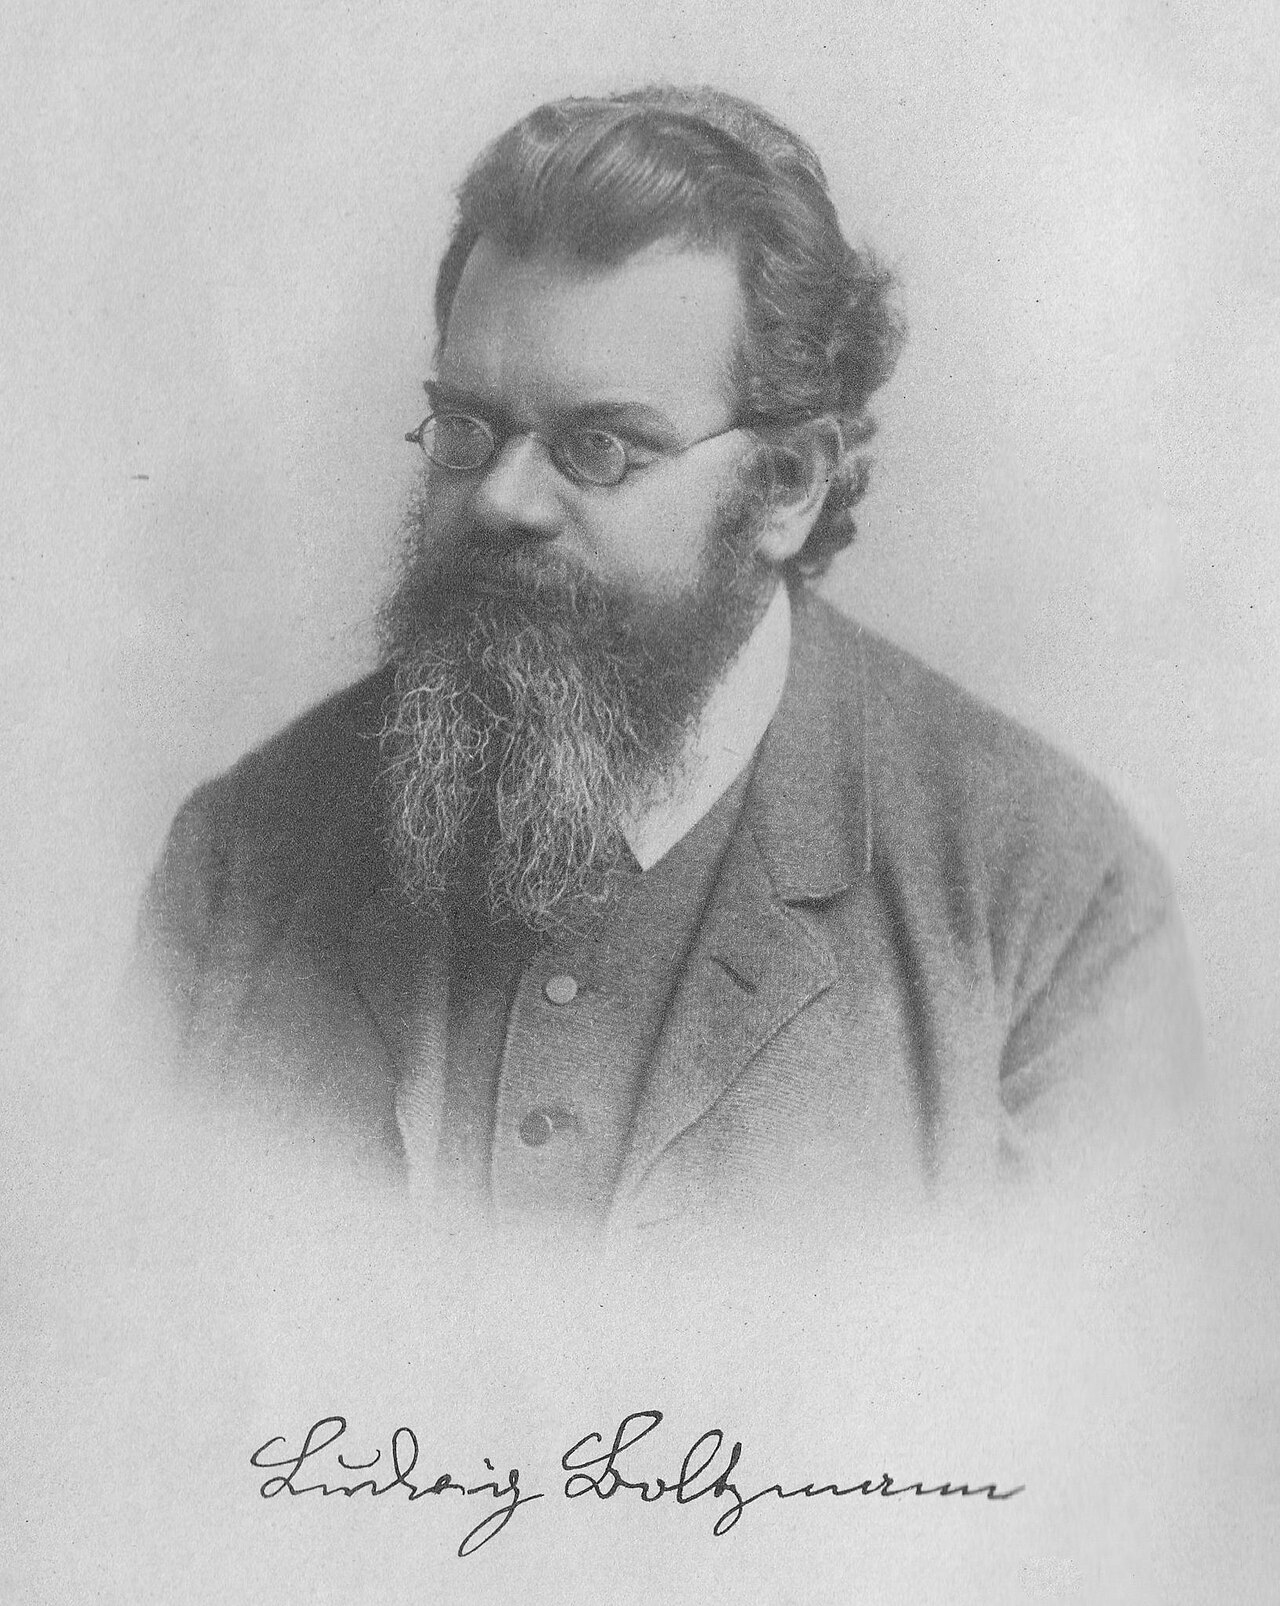
\includegraphics[width=0.3\linewidth]{images/book4/boltzmann-portrait.jpg}

{\small لودفيغ بولتزمان (1844--1906)، وعامله $\eu^{-E/k_BT}$ موضوع هذا الفصل، وصيغته $S = k_B\ln\Omega$ منقوشة على قبره في فيينا.}
\end{omfigure}

\section{مسألة: الجوّ متساوي الحرارة، وإفلات الهليوم، ومقياس حرارة سبيني}

\begin{problem}[{مسألة نهاية الأسبوع --- ثلاثة استعمالات لأسّية واحدة}]\label{pb:b2:boltzmann-factor:1}
المعطيات: $k_B = \qty{1.38e-23}{J/K}$، و $N_A = \qty{6.02e23}{mol^{-1}}$، و $g =
\qty{9.8}{m/s^2}$، و $R_{\oplus} = \qty{6.37e6}{m}$، و $\mu_B = \qty{9.27e-24}{J/T}$؛
والهواء $M = \qty{29}{g/mol}$، والهليوم \qty{4}{g/mol}، والآزوت \qty{28}{g/mol}.

\textbf{الجزء الأول --- الجوّ متساوي الحرارة.}
\begin{enumerate}
  \item من الهيدروستاتيك وقانون الغاز المثالي، استنتج $P(z) =
        P_0\eu^{-z/H}$ وأعطِ $H$ للهواء عند \qty{288}{K}.
  \item وعيّن عامل بولتزمان في النتيجة؛ فأي طاقة،
        وأي حرارة؟
  \item والضغط عند \qty{3000}{m}، و \qty{5500}{m}، و \qty{8849}{m}؛ والارتفاع
        الذي ينتصف عنده الضغط.
  \item وكتلة الجوّ في المتر المربع (من $P_0 =
        \qty{1.013e5}{Pa}$)، والكتلة الكلية؛ وتحقق من أن $\int_0^\infty
        \rho\,\dd z = \rho_0H$.
  \item وعدد الجزيئات في الجوّ.
  \item ولو تبع كل غاز ارتفاع سلّمه $H$، فما كانت تكون نسبة
        O$_2$ إلى N$_2$ عند \qty{50}{km} بالقياس إلى الأرض؟ ولمَ يكون
        التركيب منتظمًا في الواقع حتى \qty{100}{km}؟
  \item والتروبوسفير الحقيقي يبرد \qty{6.5}{K/km}: أيكون الضغط
        عند \qty{10}{km} أعلى أم أدنى من التقدير متساوي الحرارة؟
        فسّر.
  \item \omterm{def:b2:particle-diffusion:flux}{والكثافة العددية} عند مستوى البحر وعند \qty{100}{km} (بالنموذج
        متساوي الحرارة، \qty{288}{K}): علّق على ``حرف الفضاء''.
\end{enumerate}

\textbf{الجزء الثاني --- إفلات الهليوم.}
الغلاف الخارجي، فوق \qty{500}{km}، عند نحو \qty{1000}{K} و
بلا تصادمات: فالجزيء المتحرك صاعدًا أسرع من سرعة الإفلات
يغادر.
\begin{enumerate}[resume]
  \item أوجد سرعة الإفلات من الأرض عند ذلك الارتفاع.
  \item والسرعتين الأرجح والوسطى للهليوم والآزوت عند
        \qty{1000}{K}.
  \item ونسبة ذرات الهليوم التي $v > v_{\text{إفلات}}$ (استعمل
        $(2/\sqrt\pi)x\eu^{-x^2}$)؛ والنسبة نفسها للآزوت.
  \item وتدفق الهليوم المفلت نحو $\tfrac14n_{\text{He}}\langle
        v\rangle \times$ (تلك النسبة) $\times\tfrac12$؛ ومع $n_{\text{He}}
        = \qty{1e12}{m^{-3}}$ عند قاعدة الغلاف الخارجي، قدّر الضياع في المتر
        المربع في الثانية وفي السنة للأرض كلها.
  \item والهليوم في الهواء \qty{5}{ppm} حجمًا: أوجد الهليوم الكلي في
        الجوّ؛ وزمن مكوثه في وجه الضياع المحسوب.
  \item والنشاط الإشعاعي في القشرة ينتج نحو \qty{3e6}{kg} من الهليوم
        في السنة: أيكون هليوم الجوّ في حالة مستقرة، وماذا
        تعلّم المقارنة بالسؤال 11؟
  \item وعند العظم الشمسي يبلغ الغلاف الخارجي \qty{2000}{K}: بأي
        عامل ترتفع نسبة إفلات الهليوم؟
  \item ولمَ لا جوّ للقمر، ولتيتان (سرعة إفلاته
        \qty{2.6}{km/s}، و \qty{94}{K}) جوّ كثيف؟
\end{enumerate}

\textbf{الجزء الثالث --- مقياس حرارة سبيني.}
يحوي ملح بارامغناطيسي $n = \qty{2e27}{m^{-3}}$ سبينًا نصفيًّا مع $\mu
= \mu_B$، في حقل $B$.
\begin{enumerate}[resume]
  \item أوجد جمهرتي المستويين والمغنطة
        $M(B,T)$.
  \item وعند $B = \qty{0.1}{T}$: أوجد $M$ عند \qty{300}{K}، و \qty{4}{K}، و \qty{0.05}{K}؛
        وأين يصحّ \omterm{prop:b2:boltzmann-factor:curie}{قانون كوري}؟
  \item ولمَ تكون $M$ مقياس حرارة، وفي أي مجال تكون أشدّ
        حساسية؟ وماذا يُقاس عمليًّا؟
  \item ومتوسط طاقة السبينات وسعتها الحرارية (شوتكي)؛
        وحرارة القمة عند \qty{0.1}{T}.
  \item وإنتروبيا السبينات عند الحرارة العالية وعند الصفر؛ وأي
        ``ترتيب'' يقع كلما $T \to 0$؟
  \item وإزالة المغنطة الكظومة من \qty{1}{K} و \qty{1}{T} إلى \qty{0.01}{T}:
        أوجد الحرارة النهائية؛ ولمَ لا يعطي $B \to 0$ أن $T \to 0$؟
  \item ومقياس حرارة بالسبين النووي يستعمل $\mu_{\text{N}} = \mu_B/1836$: عند
        \qty{1}{T}، إلى أي حرارة يصحّ \omterm{prop:b2:boltzmann-factor:curie}{قانون كوري}، و
        لمَ يُستعمل مقياس كهذا في مجال الميكروكلفن؟
  \item وقارن عرض دوبلر لخط طيفي (من توزيع ماكسويل)
        مقياسَ حرارة للغازات: فأي مقدار، وكيف
        يتغير مع $T$؟
  \item ولخّص: الأنظمة الثلاثة والصيغة الواحدة.
\end{enumerate}
\end{problem}
